\begin{tikzpicture}[scale = 0.8]
	\coordinate (c0) at (0, 0);
	\coordinate (c1) at (3, 0);
	\coordinate (c2) at (6, 0);
	\coordinate (c3a) at (9, 2);
	\coordinate (c3b) at (9, 0);
	\coordinate (c3c) at (9, -2);
	
	\node at (c0) {\begin{tikzpicture}

\node at (0,0) [draw, scale = 5]{};
\node at (0, 0.3) {\scriptsize{\texttt{0xBC...}}};
\node at (0, 0) {\scriptsize{\texttt{0xA6...}}};
\node at (0, -0.3) {\scriptsize{\texttt{0x62...}}};

\end{tikzpicture}};
	\node at (c1) {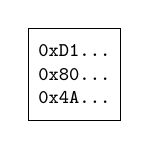
\begin{tikzpicture}

\node at (0,0) [draw, scale = 5]{};
\node at (0, 0.3) {\scriptsize{\texttt{0xD1...}}};
\node at (0, 0) {\scriptsize{\texttt{0x80...}}};
\node at (0, -0.3) {\scriptsize{\texttt{0x4A...}}};

\end{tikzpicture}};
	\node at (c2) {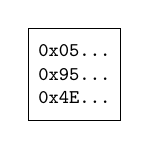
\begin{tikzpicture}

\node at (0,0) [draw, scale = 5]{};
\node at (0, 0.3) {\scriptsize{\texttt{0x05...}}};
\node at (0, 0) {\scriptsize{\texttt{0x95...}}};
\node at (0, -0.3) {\scriptsize{\texttt{0x4E...}}};

\end{tikzpicture}};
	
	\node at (c3a) {\input{../assets/figures/block_order3a.tex}};
	\node at (c3b) {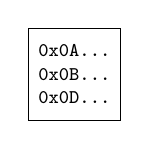
\begin{tikzpicture}

\node at (0,0) [draw, scale = 5]{};
\node at (0, 0.3) {\scriptsize{\texttt{0x0A...}}};
\node at (0, 0) {\scriptsize{\texttt{0x0B...}}};
\node at (0, -0.3) {\scriptsize{\texttt{0x0D...}}};

\end{tikzpicture}};
	\node at (c3c) {\input{../assets/figures/block_order3c.tex}};

	\draw[dotted, thick] ([xshift = 25pt]c0) -- ([xshift = -25pt]c1);
	\draw[dotted, thick] ([xshift = 25pt]c1) -- ([xshift = -25pt]c2);
	\draw[dotted, thick] ([xshift = 25pt]c2) -- ([xshift = -25pt]c3a);
	\draw[dotted, thick] ([xshift = 25pt]c2) -- ([xshift = -25pt]c3b);
	\draw[dotted, thick] ([xshift = 25pt]c2) -- ([xshift = -25pt]c3c);

\end{tikzpicture}